\documentclass[12pt,letterpaper]{article}

% ── Packages ──────────────────────────────────────────────────────────────────
\usepackage[top=0.75in, bottom=0.75in, left=0.8in, right=0.8in]{geometry}
\usepackage{amsmath, amssymb}
\usepackage{enumitem}
\usepackage{array}
\usepackage{booktabs}
\usepackage{tabularx}
\usepackage{multicol}
\usepackage{tikz}
\usepackage{pgfplots}
\pgfplotsset{compat=1.18}
\usepackage{mdframed}
\usepackage{xcolor}
\usepackage{fancyhdr}
\usepackage[T1]{fontenc}
\usepackage{parskip}
\usepackage{tcolorbox}
\tcbuselibrary{skins, breakable}
\usepackage{tasks}

% ── Colors ────────────────────────────────────────────────────────────────────
\definecolor{navyblue}{RGB}{44,62,122}
\definecolor{lightblue}{RGB}{238,242,251}
\definecolor{answergreen}{RGB}{34,100,34}

% ── Section command (no titlesec — fully portable) ────────────────────────────
\newcounter{sectionnum}
\newcommand{\worksheetsection}[1]{%
  \stepcounter{sectionnum}%
  \vspace{10pt}%
  \noindent\colorbox{navyblue}{%
    \parbox{\dimexpr\linewidth-2\fboxsep\relax}{%
      \strut\color{white}\bfseries\large
      Section \thesectionnum: #1%
    }%
  }%
  \par\vspace{4pt}%
}

% ── Subsection style (no titlesec) ────────────────────────────────────────────
\newcommand{\worksheetsubsection}[1]{%
  \vspace{4pt}%
  {\noindent\small\bfseries\color{navyblue}#1}\par\vspace{2pt}%
}

% ── Example box ───────────────────────────────────────────────────────────────
\tcbset{
  examplebox/.style={
    colback=lightblue,
    colframe=navyblue,
    leftrule=4pt, toprule=0.5pt, bottomrule=0.5pt, rightrule=0.5pt,
    arc=3pt,
    fonttitle=\bfseries\small\color{navyblue},
    title=\textbf{Example},
    before skip=6pt, after skip=8pt,
    left=8pt, right=8pt, top=6pt, bottom=6pt
  },
  answerbox/.style={
    colback=white,
    colframe=navyblue!40,
    arc=2pt,
    left=6pt, right=6pt, top=4pt, bottom=4pt,
    before skip=4pt, after skip=6pt
  }
}

% ── Work space box ────────────────────────────────────────────────────────────
\newcommand{\workbox}[1][2.0cm]{%
  \vspace{3pt}%
  \begin{tcolorbox}[
    colback=gray!5, colframe=gray!40, arc=2pt,
    left=4pt, right=4pt, top=2pt, bottom=2pt,
    height=#1, valign=top
  ]%
  \textcolor{gray!50}{\tiny Work space}%
  \end{tcolorbox}%
  \vspace{2pt}%
}

% ── Graph box ─────────────────────────────────────────────────────────────────
\newcommand{\graphbox}{%
  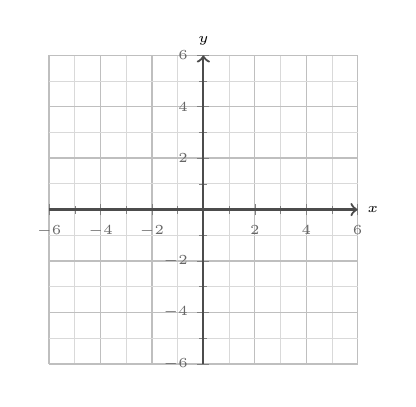
\begin{tikzpicture}
    \begin{axis}[
      width=5.5cm, height=5.5cm,
      xmin=-6, xmax=6, ymin=-6, ymax=6,
      xtick={-6,-4,...,6}, ytick={-6,-4,...,6},
      minor tick num=1,
      grid=both,
      grid style={line width=0.3pt, draw=gray!30},
      major grid style={line width=0.5pt, draw=gray!50},
      axis lines=center,
      axis line style={->, thick, color=black!70},
      tick style={very thin, color=black!50},
      ticklabel style={font=\tiny, color=black!60},
      xlabel={$x$}, ylabel={$y$},
      xlabel style={font=\tiny, at={(axis description cs:1,0.5)}, anchor=west},
      ylabel style={font=\tiny, at={(axis description cs:0.5,1)}, anchor=south},
    ]
    \end{axis}
  \end{tikzpicture}%
}

% ── Key features table ────────────────────────────────────────────────────────
\newcommand{\featurebox}{%
  \renewcommand{\arraystretch}{1.9}%
  \begin{tabular}{@{}p{3.2cm}p{4.5cm}@{}}
    Vertex:              & \hrulefill \\
    Axis of Symmetry:    & \hrulefill \\
    Domain:              & \hrulefill \\
    Range:               & \hrulefill \\
    Opens:               & Up \quad Down \\
  \end{tabular}%
}

% ── Header/footer ─────────────────────────────────────────────────────────────
\pagestyle{fancy}
\fancyhf{}
\renewcommand{\headrulewidth}{0pt}
\fancyfoot[C]{\small\color{gray!70} Algebra 1 Comprehensive Review \quad|\quad \thepage}

% ── Misc ──────────────────────────────────────────────────────────────────────
\setlength{\parindent}{0pt}
\setlist[enumerate]{topsep=2pt, itemsep=4pt, parsep=0pt}
\setlist[itemize]{topsep=2pt, itemsep=2pt}

% ══════════════════════════════════════════════════════════════════════════════
\begin{document}

% ── Title block ───────────────────────────────────────────────────────────────
\begin{tcolorbox}[
  colback=navyblue, colframe=navyblue,
  arc=4pt, boxrule=0pt,
  left=10pt, right=10pt, top=8pt, bottom=8pt,
  halign=center
]
  {\Large\bfseries\color{white} Algebra 1 \textemdash{} Comprehensive Review Worksheet}\\[4pt]
  {\small\color{white!85!navyblue}
    Factoring $\cdot$ Completing the Square $\cdot$ Graphing Quadratics
    $\cdot$ Sequences $\cdot$ Exponential Transformations}
\end{tcolorbox}
\vspace{10pt}

% ── Student info ──────────────────────────────────────────────────────────────
\noindent
\begin{tabular*}{\linewidth}{@{}l@{\extracolsep{16pt}}l@{\extracolsep{16pt}}l@{\extracolsep{\fill}}r@{}}
  \textbf{Name:}~\underline{\hspace{5cm}} &
  \textbf{Date:}~\underline{\hspace{3cm}} &
  \textbf{Period:}~\underline{\hspace{2cm}} &
  \textbf{Score:}~\underline{\hspace{1.2cm}}~/~50
\end{tabular*}
\vspace{12pt}

% ══════════════════════════════════════════════════════════════════════════════
\worksheetsection{Solving Equations by Factoring}

\begin{tcolorbox}[examplebox]
  Solve:\quad $x^2 + 5x + 6 = 0$\\[4pt]
  \textbf{Step 1.} Find two numbers that multiply to $6$ and add to $5$ $\longrightarrow$ $2$ and $3$\\
  \textbf{Step 2.} Factor:\quad $(x+2)(x+3)=0$\\
  \textbf{Step 3.} Zero Product Property:\quad $x+2=0 \;\Rightarrow\; \boldsymbol{x=-2}$\qquad $x+3=0 \;\Rightarrow\; \boldsymbol{x=-3}$
\end{tcolorbox}

\worksheetsubsection{A.\ Multiple Choice} \textit{(Circle the best answer.)}

\begin{enumerate}[label=\textbf{\arabic*.}, leftmargin=*, itemsep=10pt]

  \item Solve: $x^2 + 7x + 12 = 0$
  \begin{tasks}(4)
    \task $x=3,\;4$
    \task $x=-3,\;-4$
    \task $x=-3,\;4$
    \task $x=3,\;-4$
  \end{tasks}

  \item Solve: $x^2 - 5x + 6 = 0$
  \begin{tasks}(4)
    \task $x=-2,\;-3$
    \task $x=2,\;3$
    \task $x=-2,\;3$
    \task $x=2,\;-3$
  \end{tasks}

  \item Solve: $x^2 - 9 = 0$
  \begin{tasks}(4)
    \task $x=9$
    \task $x=3$
    \task $x=\pm 3$
    \task $x=\pm 9$
  \end{tasks}

  \item Solve: $2x^2 + 5x + 2 = 0$
  \begin{tasks}(4)
    \task $x=-\tfrac{1}{2},\;-2$
    \task $x=\tfrac{1}{2},\;2$
    \task $x=-\tfrac{1}{2},\;2$
    \task $x=\tfrac{1}{2},\;-2$
  \end{tasks}

  \item Solve: $x^2 - x - 12 = 0$
  \begin{tasks}(4)
    \task $x=-4,\;3$
    \task $x=4,\;-3$
    \task $x=4,\;3$
    \task $x=-4,\;-3$
  \end{tasks}

\end{enumerate}

\vspace{6pt}
\worksheetsubsection{B.\ Practice Problems} \textit{(Show all work.)}

\begin{enumerate}[label=\textbf{\arabic*.}, leftmargin=*, itemsep=4pt]
  \item Solve:\quad $x^2 + 8x + 15 = 0$ \workbox
  \item Solve:\quad $x^2 - 6x + 8 = 0$ \workbox
  \item Solve:\quad $x^2 - 25 = 0$ \workbox
  \item Solve:\quad $3x^2 + 7x + 2 = 0$ \workbox
  \item Solve:\quad $x^2 + 2x - 15 = 0$ \workbox
\end{enumerate}

\newpage
% ══════════════════════════════════════════════════════════════════════════════
\worksheetsection{Solving Equations by Completing the Square}

\begin{tcolorbox}[examplebox]
  Solve:\quad $x^2 + 6x + 5 = 0$\\[4pt]
  \textbf{Step 1.} Move constant:\quad $x^2 + 6x = -5$\\
  \textbf{Step 2.} Add $\left(\dfrac{6}{2}\right)^2 = 9$ to both sides:\quad $x^2 + 6x + 9 = 4$\\[2pt]
  \textbf{Step 3.} Perfect square:\quad $(x+3)^2 = 4$\\
  \textbf{Step 4.} Square root:\quad $x+3 = \pm 2 \;\Rightarrow\; \boldsymbol{x = -1}$ \quad or\quad $\boldsymbol{x=-5}$
\end{tcolorbox}

\worksheetsubsection{A.\ Multiple Choice} \textit{(Circle the best answer.)}

\begin{enumerate}[label=\textbf{\arabic*.}, leftmargin=*, itemsep=10pt]

  \item Solve by completing the square: $x^2 + 4x - 5 = 0$
  \begin{tasks}(4)
    \task $x=1,\;-5$
    \task $x=-1,\;5$
    \task $x=1,\;5$
    \task $x=-1,\;-5$
  \end{tasks}

  \item Solve: $x^2 - 6x + 5 = 0$
  \begin{tasks}(4)
    \task $x=-1,\;-5$
    \task $x=1,\;5$
    \task $x=2,\;3$
    \task $x=-2,\;-3$
  \end{tasks}

  \item What number completes the square for $x^2 + 10x + \underline{\hspace{1cm}}$\,?
  \begin{tasks}(4)
    \task $5$
    \task $10$
    \task $25$
    \task $100$
  \end{tasks}

  \item Solve: $x^2 - 8x + 7 = 0$
  \begin{tasks}(4)
    \task $x=1,\;7$
    \task $x=-1,\;-7$
    \task $x=2,\;4$
    \task $x=-2,\;-4$
  \end{tasks}

  \item Solve: $x^2 + 2x - 3 = 0$
  \begin{tasks}(4)
    \task $x=-3,\;1$
    \task $x=3,\;-1$
    \task $x=3,\;1$
    \task $x=-3,\;-1$
  \end{tasks}

\end{enumerate}

\vspace{6pt}
\worksheetsubsection{B.\ Practice Problems} \textit{(Show all work.)}

\begin{enumerate}[label=\textbf{\arabic*.}, leftmargin=*, itemsep=4pt]
  \item Solve by completing the square:\quad $x^2 + 6x + 8 = 0$ \workbox
  \item Solve by completing the square:\quad $x^2 - 4x - 12 = 0$ \workbox
  \item Solve by completing the square:\quad $x^2 + 8x + 12 = 0$ \workbox
  \item Solve by completing the square:\quad $x^2 - 10x + 16 = 0$ \workbox
  \item Solve by completing the square:\quad $x^2 + 12x + 20 = 0$ \workbox
\end{enumerate}

\newpage
% ══════════════════════════════════════════════════════════════════════════════
\worksheetsection{Graphing Quadratic Equations}

\begin{tcolorbox}[examplebox]
  Graph $y = x^2 - 4x + 3$ and identify all key features.\\[4pt]
  \textbf{Axis of Symmetry:}\quad $x = -\dfrac{b}{2a} = -\dfrac{-4}{2(1)} = 2$\\[4pt]
  \textbf{Vertex:}\quad $y = (2)^2 - 4(2) + 3 = -1 \;\Rightarrow\; \textbf{Vertex} = (2,\,-1)$\\
  \textbf{$y$-intercept:} $(0,\,3)$ \qquad \textbf{$x$-intercepts:} $(x-1)(x-3)=0 \Rightarrow x=1,\;x=3$\\
  \textbf{Domain:} $-\infty < x < \infty$ \qquad \textbf{Range:} $y \ge -1$
\end{tcolorbox}

\worksheetsubsection{A.\ Multiple Choice} \textit{(Circle the best answer.)}

\begin{enumerate}[label=\textbf{\arabic*.}, leftmargin=*, itemsep=10pt]

  \item For $y = x^2 - 6x + 5$, what is the vertex?
  \begin{tasks}(4)
    \task $(3,\,-4)$
    \task $(-3,\,4)$
    \task $(3,\,4)$
    \task $(6,\,5)$
  \end{tasks}

  \item What is the axis of symmetry for $y = 2x^2 + 8x - 1$?
  \begin{tasks}(4)
    \task $x=4$
    \task $x=-4$
    \task $x=-2$
    \task $x=2$
  \end{tasks}

  \item What is the range of $y = x^2 + 2$?
  \begin{tasks}(4)
    \task $y \ge 0$
    \task $y \ge 2$
    \task all reals
    \task $y \le 2$
  \end{tasks}

  \item Which parabola opens downward?
  \begin{tasks}(4)
    \task $y = 3x^2$
    \task $y = x^2-5$
    \task $y = -2x^2+1$
    \task $y = (x-1)^2$
  \end{tasks}

  \item The domain of ANY quadratic $y = ax^2+bx+c$ is:
  \begin{tasks}(4)
    \task $x \ge 0$
    \task $x \le 0$
    \task all reals
    \task depends on $a$
  \end{tasks}

\end{enumerate}

\vspace{6pt}
\worksheetsubsection{B.\ Practice Problems} \textit{(Graph each parabola and identify all key features.)}

\begin{enumerate}[label=\textbf{\arabic*.}, leftmargin=*, itemsep=10pt]

  \item $y = x^2 - 2x - 3$\\[4pt]
  \begin{minipage}[t]{5.8cm}\graphbox\end{minipage}\hfill
  \begin{minipage}[t]{7.5cm}\vspace{6pt}\featurebox\end{minipage}

  \item $y = -x^2 + 4x$\\[4pt]
  \begin{minipage}[t]{5.8cm}\graphbox\end{minipage}\hfill
  \begin{minipage}[t]{7.5cm}\vspace{6pt}\featurebox\end{minipage}

  \item $y = x^2 + 4x + 4$\\[4pt]
  \begin{minipage}[t]{5.8cm}\graphbox\end{minipage}\hfill
  \begin{minipage}[t]{7.5cm}\vspace{6pt}\featurebox\end{minipage}

  \item $y = 2x^2 - 8x + 6$\\[4pt]
  \begin{minipage}[t]{5.8cm}\graphbox\end{minipage}\hfill
  \begin{minipage}[t]{7.5cm}\vspace{6pt}\featurebox\end{minipage}

  \item $y = -x^2 + 6x - 5$\\[4pt]
  \begin{minipage}[t]{5.8cm}\graphbox\end{minipage}\hfill
  \begin{minipage}[t]{7.5cm}\vspace{6pt}\featurebox\end{minipage}

\end{enumerate}

\newpage
% ══════════════════════════════════════════════════════════════════════════════
\worksheetsection{Arithmetic \& Geometric Sequences --- The $n$th Term}

\begin{tcolorbox}[examplebox]
  \textbf{Arithmetic} (add constant difference $d$):\quad $a_n = a_1 + (n-1)d$\\
  \quad Sequence: $3,\;7,\;11,\;15,\;\ldots$ \quad $a_1=3,\;d=4$
  \quad $\Rightarrow$ \quad $a_n = 3+(n-1)\cdot 4 = \boldsymbol{4n-1}$\\[6pt]
  \textbf{Geometric} (multiply by constant ratio $r$):\quad $a_n = a_1 \cdot r^{n-1}$\\
  \quad Sequence: $2,\;6,\;18,\;54,\;\ldots$ \quad $a_1=2,\;r=3$
  \quad $\Rightarrow$ \quad $a_n = \boldsymbol{2\cdot 3^{n-1}}$
\end{tcolorbox}

\worksheetsubsection{A.\ Multiple Choice} \textit{(Circle the best answer.)}

\begin{enumerate}[label=\textbf{\arabic*.}, leftmargin=*, itemsep=10pt]

  \item Find the 10th term of the arithmetic sequence: $5,\;9,\;13,\;17,\;\ldots$
  \begin{tasks}(4)
    \task $40$
    \task $41$
    \task $45$
    \task $36$
  \end{tasks}

  \item Find the $n$th term formula for: $2,\;5,\;8,\;11,\;\ldots$
  \begin{tasks}(4)
    \task $a_n = 3n-1$
    \task $a_n = 3n+2$
    \task $a_n = 2n+1$
    \task $a_n = n+3$
  \end{tasks}

  \item Find the 5th term of the geometric sequence: $3,\;6,\;12,\;24,\;\ldots$
  \begin{tasks}(4)
    \task $48$
    \task $96$
    \task $36$
    \task $192$
  \end{tasks}

  \item Which sequence is geometric?
  \begin{tasks}(4)
    \task $2,\;4,\;6,\;8$
    \task $1,\;3,\;6,\;10$
    \task $4,\;12,\;36,\;108$
    \task $5,\;10,\;15,\;20$
  \end{tasks}

  \item The formula $a_n = 2\cdot 4^{n-1}$ describes which type of sequence?
  \begin{tasks}(4)
    \task Arithmetic, $d=4$
    \task Geometric, $r=4$
    \task Geometric, $r=2$
    \task Arithmetic, $d=2$
  \end{tasks}

\end{enumerate}

\vspace{6pt}
\worksheetsubsection{B.\ Practice Problems} \textit{(Show all work.)}

\begin{enumerate}[label=\textbf{\arabic*.}, leftmargin=*, itemsep=4pt]
  \item Write the $n$th term formula and find $a_{12}$ for: $7,\;11,\;15,\;19,\;\ldots$ \workbox
  \item Write the $n$th term formula and find $a_6$ for the geometric sequence: $5,\;15,\;45,\;135,\;\ldots$ \workbox
  \item Find the 20th term: $-3,\;1,\;5,\;9,\;\ldots$ \workbox
  \item A geometric sequence has $a_1=100$ and $r=\tfrac{1}{2}$. Write the $n$th term formula and find $a_5$. \workbox
  \item Is the sequence $64,\;32,\;16,\;8,\;\ldots$ arithmetic or geometric? Write the $n$th term formula. \workbox
\end{enumerate}

\newpage
% ══════════════════════════════════════════════════════════════════════════════
\worksheetsection{Transformations of Exponential Functions}

\begin{tcolorbox}[examplebox]
  \textbf{Parent function:} $f(x) = 2^x$ \qquad
  \textbf{General form:} $g(x) = a\cdot b^{x-h} + k$\\[4pt]
  \begin{tabular}{@{}ll@{}}
    $|a|>1$                   & vertical stretch \\
    $0<|a|<1$                 & vertical compression \\
    $a<0$                     & reflection over the $x$-axis \\
    replace $x$ with $-x$     & reflection over the $y$-axis \\
    $h>0$                     & shift right $h$ units \\
    $h<0$                     & shift left $|h|$ units \\
    $k>0$                     & shift up $k$ units \\
    $k<0$                     & shift down $|k|$ units \\
  \end{tabular}\\[6pt]
  \textbf{Example:}\quad $g(x) = -3\cdot 2^{x+2} - 1$ $\Rightarrow$
  reflect over $x$-axis, vertical stretch $\times 3$, left $2$, down $1$.
  \quad Asymptote: $y=-1$
\end{tcolorbox}

\worksheetsubsection{A.\ Multiple Choice} \textit{(Circle the best answer.)}

\begin{enumerate}[label=\textbf{\arabic*.}, leftmargin=*, itemsep=10pt]

  \item How does $g(x)=2^x+5$ compare to $f(x)=2^x$?
  \begin{tasks}(4)
    \task Shift left 5
    \task Shift right 5
    \task Shift up 5
    \task Shift down 5
  \end{tasks}

  \item Describe the transformation: $g(x)=2^{x-3}$
  \begin{tasks}(4)
    \task Shift up 3
    \task Shift down 3
    \task Shift left 3
    \task Shift right 3
  \end{tasks}

  \item Which equation represents a vertical stretch by a factor of 4 of $f(x)=3^x$?
  \begin{tasks}(4)
    \task $f(x)=3^{4x}$
    \task $f(x)=4\cdot 3^x$
    \task $f(x)=3^x+4$
    \task $f(x)=\tfrac{1}{4}\cdot 3^x$
  \end{tasks}

  \item What is the horizontal asymptote of $g(x)=2^x - 7$?
  \begin{tasks}(4)
    \task $y=2$
    \task $y=7$
    \task $y=-7$
    \task $y=0$
  \end{tasks}

  \item $g(x)=-2^x$ is a reflection of $f(x)=2^x$ over which axis?
  \begin{tasks}(4)
    \task $y$-axis
    \task $x$-axis
    \task the origin
    \task the line $y=x$
  \end{tasks}

\end{enumerate}

\vspace{6pt}
\worksheetsubsection{B.\ Practice Problems} \textit{(Describe all transformations fully.)}

\begin{enumerate}[label=\textbf{\arabic*.}, leftmargin=*, itemsep=4pt]
  \item Describe all transformations:\quad $g(x) = 3\cdot 2^{x-1} + 4$ \workbox
  \item Write the equation of $f(x)=4^x$ shifted \textbf{left 2}, reflected over the $x$-axis, and shifted \textbf{down 3}. \workbox
  \item State the domain, range, and asymptote of\quad $g(x) = -2\cdot 5^x + 1$ \workbox
  \item Describe all transformations:\quad $g(x) = \tfrac{1}{2}\cdot 3^{-x} - 2$ \workbox
  \item The graph of $f(x)=2^x$ is transformed to pass through $(0,\,6)$ with asymptote $y=-1$.\\
        Write a possible equation in the form $g(x)=a\cdot 2^x + k$. \workbox
\end{enumerate}

% ══════════════════════════════════════════════════════════════════════════════
% ANSWER KEY
% ══════════════════════════════════════════════════════════════════════════════
\newpage
\begin{center}
  {\color{navyblue}\rule{\linewidth}{2pt}}\\[6pt]
  {\Large\bfseries\color{navyblue} Answer Key}\\[4pt]
  {\small Total: 50 points \quad|\quad Multiple Choice: 25 pts (1 pt each) \quad|\quad Practice: 25 pts (1 pt each)}\\[4pt]
  {\color{navyblue}\rule{\linewidth}{2pt}}
\end{center}

% ── Section 1 ─────────────────────────────────────────────────────────────────
\textbf{\color{navyblue}Section 1 --- Solving by Factoring}

\smallskip
\textbf{Multiple Choice:}\quad 1.\,B \quad 2.\,B \quad 3.\,C \quad 4.\,A \quad 5.\,B

\smallskip
\textbf{Practice:}
\begin{enumerate}[label=\arabic*., leftmargin=*, itemsep=3pt, topsep=2pt]
  \item $x^2+8x+15=0 \;\Rightarrow\; (x+3)(x+5)=0 \;\Rightarrow\; \boldsymbol{x=-3,\;-5}$
  \item $x^2-6x+8=0 \;\Rightarrow\; (x-2)(x-4)=0 \;\Rightarrow\; \boldsymbol{x=2,\;4}$
  \item $x^2-25=0 \;\Rightarrow\; (x-5)(x+5)=0 \;\Rightarrow\; \boldsymbol{x=\pm 5}$
  \item $3x^2+7x+2=0 \;\Rightarrow\; (3x+1)(x+2)=0 \;\Rightarrow\; \boldsymbol{x=-\tfrac{1}{3},\;-2}$
  \item $x^2+2x-15=0 \;\Rightarrow\; (x+5)(x-3)=0 \;\Rightarrow\; \boldsymbol{x=-5,\;3}$
\end{enumerate}

\vspace{6pt}
% ── Section 2 ─────────────────────────────────────────────────────────────────
\textbf{\color{navyblue}Section 2 --- Completing the Square}

\smallskip
\textbf{Multiple Choice:}\quad 1.\,A \quad 2.\,B \quad 3.\,C \quad 4.\,A \quad 5.\,A

\smallskip
\textbf{Practice:}
\begin{enumerate}[label=\arabic*., leftmargin=*, itemsep=3pt, topsep=2pt]
  \item $x^2+6x+8=0 \;\Rightarrow\; (x+3)^2=1 \;\Rightarrow\; \boldsymbol{x=-2,\;-4}$
  \item $x^2-4x-12=0 \;\Rightarrow\; (x-2)^2=16 \;\Rightarrow\; \boldsymbol{x=6,\;-2}$
  \item $x^2+8x+12=0 \;\Rightarrow\; (x+4)^2=4 \;\Rightarrow\; \boldsymbol{x=-2,\;-6}$
  \item $x^2-10x+16=0 \;\Rightarrow\; (x-5)^2=9 \;\Rightarrow\; \boldsymbol{x=8,\;2}$
  \item $x^2+12x+20=0 \;\Rightarrow\; (x+6)^2=16 \;\Rightarrow\; \boldsymbol{x=-2,\;-10}$
\end{enumerate}

\vspace{6pt}
% ── Section 3 ─────────────────────────────────────────────────────────────────
\textbf{\color{navyblue}Section 3 --- Graphing Quadratics}

\smallskip
\textbf{Multiple Choice:}\quad 1.\,A \quad 2.\,C \quad 3.\,B \quad 4.\,C \quad 5.\,C

\smallskip
\textbf{Practice:}
\begin{enumerate}[label=\arabic*., leftmargin=*, itemsep=3pt, topsep=2pt]
  \item $y=x^2-2x-3$: Vertex $\boldsymbol{(1,-4)}$, AOS $x=1$, Domain: all reals, Range: $y\ge -4$, Opens up
  \item $y=-x^2+4x$: Vertex $\boldsymbol{(2,4)}$, AOS $x=2$, Domain: all reals, Range: $y\le 4$, Opens down
  \item $y=x^2+4x+4$: Vertex $\boldsymbol{(-2,0)}$, AOS $x=-2$, Domain: all reals, Range: $y\ge 0$, Opens up
  \item $y=2x^2-8x+6$: Vertex $\boldsymbol{(2,-2)}$, AOS $x=2$, Domain: all reals, Range: $y\ge -2$, Opens up
  \item $y=-x^2+6x-5$: Vertex $\boldsymbol{(3,4)}$, AOS $x=3$, Domain: all reals, Range: $y\le 4$, Opens down
\end{enumerate}

\vspace{6pt}
% ── Section 4 ─────────────────────────────────────────────────────────────────
\textbf{\color{navyblue}Section 4 --- Sequences}

\smallskip
\textbf{Multiple Choice:}\quad 1.\,B \quad 2.\,A \quad 3.\,A \quad 4.\,C \quad 5.\,B

\smallskip
\textbf{Practice:}
\begin{enumerate}[label=\arabic*., leftmargin=*, itemsep=3pt, topsep=2pt]
  \item $d=4$;\quad $a_n=4n+3$;\quad $\boldsymbol{a_{12}=51}$
  \item $r=3$;\quad $a_n=5\cdot 3^{n-1}$;\quad $\boldsymbol{a_6=1215}$
  \item $d=4$;\quad $a_n=4n-7$;\quad $\boldsymbol{a_{20}=73}$
  \item $a_n=100\cdot\bigl(\tfrac{1}{2}\bigr)^{n-1}$;\quad $\boldsymbol{a_5=6.25}$
  \item \textbf{Geometric}, $r=\tfrac{1}{2}$;\quad $a_n=64\cdot\bigl(\tfrac{1}{2}\bigr)^{n-1}$
\end{enumerate}

\vspace{6pt}
% ── Section 5 ─────────────────────────────────────────────────────────────────
\textbf{\color{navyblue}Section 5 --- Exponential Transformations}

\smallskip
\textbf{Multiple Choice:}\quad 1.\,C \quad 2.\,D \quad 3.\,B \quad 4.\,C \quad 5.\,B

\smallskip
\textbf{Practice:}
\begin{enumerate}[label=\arabic*., leftmargin=*, itemsep=3pt, topsep=2pt]
  \item Vertical stretch $\times 3$, shift right 1, shift up 4
  \item $\boldsymbol{g(x) = -4^{x+2} - 3}$
  \item Domain: all reals;\quad Range: $y < 1$;\quad Asymptote: $\boldsymbol{y=1}$
  \item Vertical compression $\times\tfrac{1}{2}$, reflection over the $y$-axis, shift down 2
  \item $g(0)=a+k=6$ and $k=-1\;\Rightarrow\; a=7$;\quad $\boldsymbol{g(x)=7\cdot 2^x-1}$
\end{enumerate}

\vspace{12pt}
\begin{center}
  \textcolor{gray}{\rule{0.5\linewidth}{0.4pt}}\\[4pt]
  \textit{\small --- End of Worksheet ---}
\end{center}

\end{document}
